\chapter{Câu hỏi ôn tập}
\begin{enumerate}[label=\bfseries Câu \arabic*:, leftmargin=1.0cm]
	\item Công thức xác định độ lớn lực tương tác tĩnh điện giữa hai điện tích điểm đặt trong chân không
	\begin{mcq}(4)
		\item $F=\dfrac{k\left|q_1q_2\right|}{r^2}.$
		\item $F=\dfrac{k\varepsilon q_1q_2}{r}$.
		\item $F=\dfrac{k\left|q_1q_2\right|}{r}.$
		\item $F=\dfrac{kq_1q_2}{\varepsilon r}.$
	\end{mcq}
\hideall{
\textbf{Đáp án A.}
}

\item Có hai điện tích điểm $q_1$ và $q_2$, chúng đẩy nhau. Khẳng định nào sau đây là đúng?
\begin{mcq}(4)
	\item $q_1>0$ và $q_2<0$.
	\item $q_1<0$ và $q_2>0$.
	\item $q_1q_2>0$.
	\item $q_1q_2<0$.
\end{mcq}
\hideall{
\textbf{Đáp án C.}\\
Hai điện tích đẩy nhau thì chúng phải tích điện cùng dấu.
}

\item Một điện tích điểm $q$ và một điện tích điểm $2q$ được đặt cách nhau một khoảng $r$. Nếu lực điện tác dụng lên điện tích $2q$ có độ lớn là $F$ thì lực điện tác dụng lên điện tích $q$ có độ lớn là
\begin{mcq}(4)
	\item $0,25F$.
	\item $0,5F$.
	\item $F$.
	\item $2F$.
\end{mcq}
\hideall{
\textbf{Đáp án C.}\\
Theo định luật III Newton, lực tương tác tĩnh điện do mỗi điện tích này gây ra cho điện tích kia sẽ cùng phương, ngược chiều và cùng độ lớn.
}

\item Vector cường độ điện trường tại mỗi điểm có chiều
\begin{mcq}
	\item cùng chiều với lực điện tác dụng lên điện tích thử dương tại điểm đó.
	\item cùng chiều với lực điện tác dụng lên điện tích thử tại điểm đó.
	\item phụ thuộc độ lớn điện tích thử.
	\item phụ thuộc vào nhiệt độ của môi trường.
\end{mcq}
\hideall{
\textbf{Đáp án A.}\\
Vector cường độ điện trường tại mỗi điểm cùng chiều với lực điện tác dụng lên điện tích thử dương tại điểm đó.
}

\item Theo định luật bảo toàn điện tích: Trong một hệ cô lập về điện
\begin{mcq}
	\item tổng đại số các điện tích không đổi.
	\item tổng độ lớn các điện tích không đổi.
	\item hiệu đại số các điện tích không đổi.
	\item tích đại số các điện tích không đổi.
\end{mcq}
\hideall{
\textbf{Đáp án A.}
}

\item Trong các đơn vị sau, đơn vị của cường độ điện trường là
\begin{mcq}(4)
	\item $\si{\volt/\meter^2}$.
	\item $\si{\volt\cdot\meter}$.
	\item $\si{\volt/\meter}$.
	\item $\si{\volt\cdot\meter^2}$.
\end{mcq}
\hideall{
\textbf{Đáp án C.}
}

\item Đường sức của điện trường đều có đặc điểm
\begin{mcq}(2)
	\item là những đường cong cách đều nhau.
	\item là những đường cong bất kì.
	\item là những đường thẳng song song cách đều nhau.
	\item là những đường thẳng bất kì.
\end{mcq}
\hideall{\textbf{Đáp án C.}\\
Đường sức điện của điện trường đều là những đường thẳng song song cách đều nhau.}

\item Công của lực điện trong sự di chuyển của điện tích $q$ trong điện trường từ điểm M đến điểm N không phụ thuộc vào yếu tố nào sau đây?
\begin{mcq}
	\item Độ lớn của cường độ điện trường.
	\item Vị trí của điểm M và điểm N.
	\item Hình dạng đường đi từ điểm M đến điểm N.
	\item Điện tích $q$.
\end{mcq}
\hideall{
\textbf{Đáp án C.}\\
Công của lực điện không phụ thuộc vào hình dạng đường đi từ điểm M đến điểm N.
}

\item Cường độ điện trường tại một điểm là
\begin{mcq}
	\item đại lượng vô hướng và tỉ lệ với tích độ lớn điện tích.
	\item đại lượng đặc trưng cho điện trường về phương diện năng lượng.
	\item đại lượng đặc trưng cho điện trường về phương diện tác dụng lực.
	\item dạng vật chất tồn tại xung quanh điện tích đứng yên.
\end{mcq}
\hideall{
\textbf{Đáp án C.}\\
Cường độ điện trường tại một điểm là đại lượng đặc trưng cho điện trường về phương diện tác dụng lực.
}


\item Khi một electron chuyển động trong điện trường đều nó sẽ chịu tác dụng của lực điện $\vec{F}$. Lực này có hướng
\begin{mcq}
	\item trùng với vector cường độ điện trường $\vec{E}$.
	\item ngược với hướng của vector cường độ điện trường $\vec{E}$.
	\item vuông góc với vector cường độ điện trường $\vec{E}$.
	\item hợp với vector cường độ điện trường một góc bất kì tuỳ theo vị trí của điện tích.
\end{mcq}
\hideall{
\textbf{Đáp án B.}\\
$$\vec{F}=q_e\vec{E}$$
Vì $q_e<0$ nên $\vec{F}\uparrow\downarrow\vec{E}$.
}

\item Hai điện tích điểm $q_1=\SI{2E-9}{\coulomb}$, $q_2=\SI{4E-9}{\coulomb}$ đặt cách nhau $\SI{3}{\centi\meter}$ trong không khí, lực tương tác giữa chúng có độ lớn 
\begin{mcq}(4)
	\item $\SI{9E-5}{\newton}$.
	\item $\SI{9E-6}{\newton}$.
	\item $\SI{8E-9}{\newton}$.
	\item $\SI{8E-5}{\newton}$.
\end{mcq}
\hideall{
\textbf{Đáp án D.}\\
Lực tương tác giữa hai điện tích điểm 
$$F=\dfrac{k\left|q_1q_2\right|}{\varepsilon r^2}=\SI{8E-5}{\newton}.$$
}

\item Cường độ điện trường gây ra bởi điện tích $Q=\SI{5E-9}{\coulomb}$ tại một điểm trong chân không cách điện tích một khoảng $\SI{10}{\centi\meter}$ có độ lớn là
\begin{mcq}(4)
	\item $E=\SI{0.45}{\volt/\meter}$.
	\item $E=\SI{0.225}{\volt/\meter}$.
	\item $E=\SI{4500}{\volt/\meter}$.
	\item $E=\SI{2250}{\volt/\meter}$.
\end{mcq}
\hideall{
\textbf{Đáp án C.}\\
Độ lớn cường độ điện trường:
$$E=\dfrac{k\left|Q\right|}{r^2}=\dfrac{\left(\SI{9E9}{\dfrac{\newton\meter^2}{\coulomb^2}}\right)\cdot\left(\SI{5E-9}{\coulomb}\right)}{\left(\SI{0.1}{\meter}\right)^2}=\SI{4500}{\volt/\meter}.$$
}

\item Khi cho một điện tích điểm chuyển động vào vùng không gian điện trường đều có vector cường độ điện trường hướng vuông góc với vận tốc ban đầu $\vec v_0$. Khi đó, quãy đạo chuyển động của hạt có dạng là
\begin{mcq}(4)
	\item đường thẳng.
	\item đường tròn.
	\item một nhánh parabol.
	\item đường gấp khúc.
\end{mcq}
\hideall{
\textbf{Đáp án C.}\\
Trong quá trình chuyển động điện tích chịu tác dụng của lực tĩnh điện hướng vuông góc với vector vận tốc ban đầu nên quỹ đạo chuyển động của điện tích là một nhánh của parabol.
}

\item Một điện tích điểm $q$ chuyển động trong điện trường theo một đường cong kín. Gọi công của lực điện trong chuyển động đó là $A$ thì
\begin{mcq}
	\item $A>0$ nếu $q>0$.
	\item $A<0$ nếu $q<0$.
	\item $A=0$ trong mọi trường hợp.
	\item $A\neq 0$ còn dấu của $A$ phụ thuộc vào chiều chuyển động. 
\end{mcq}
\hideall{
\textbf{Đáp án C.}\\
Công lực điện khi điện tích chuyển động trên một đường cong kín thì bằng không.
}

\item Đặt một điện tích thử $q=\SI{2E-6}{\coulomb}$ tại một điểm trong điện trường đều, nó chịu một lực điện có độ lớn $F=\SI{2E-3}{\newton}$ có hướng từ trái qua phải. Khi này vector cường độ điện trường có hướng và độ lớn
\begin{mcq}(2)
	\item $\SI{100}{\volt/\meter}$, từ trái sang phải.
	\item $\SI{100}{\volt/\meter}$, từ phải sang trái.
	\item $\SI{1000}{\volt/\meter}$, từ trái sang phải.
	\item $\SI{1000}{\volt/\meter}$, từ phải sang trái.
\end{mcq}
\hideall{
\textbf{Đáp án C.}\\
$$\vec{E}=\dfrac{\vec{F}}{q}$$
Vì $q>0$ nên $\vec{E}\uparrow\uparrow\vec{F}$ và độ lớn cường độ điện trường:
$$E=\dfrac{F}{\left|q\right|}=\SI{1000}{\volt/\meter}.$$
}

\item Hai điểm nằm trên một đường sức của một điện trường đều cách nhau $\SI{2}{\meter}$. Độ lớn cường độ điện trường là $\SI{1000}{\volt/\meter}$. Hiệu điện thế giữa hai điểm đó là 
\begin{mcq}(4)
	\item $\SI{500}{\volt}$.
	\item $\SI{1000}{\volt}$.
	\item $\SI{2000}{\volt}$.
	\item $\SI{1500}{\volt}$.
\end{mcq}
\hideall{
\textbf{Đáp án C.}\\
 Hiệu điện thế giữa hai điểm trên:
 $$U=Ed=\left(\SI{1000}{\volt/\meter}\right)\cdot\left(\SI{2}{\meter}\right)=\SI{2000}{\volt/\meter}.$$
}

\item Có hai bản kim loại phẳng đặt song song với nhau và cách nhau $\SI{1}{\centi\meter}$. Hiệu điện thế giữa bản dương và bản âm là $\SI{120}{\volt}$. Chọn mốc điện thế ở bản dương. Điện thế tại điểm M nằm trong khoảng giữa hai bản, cách bản âm $\SI{0.6}{\centi\meter}$ là
\begin{mcq}(4)
	\item $\SI{-48}{\volt}$.
	\item $\SI{72}{\volt}$.
	\item $\SI{48}{\volt}$.
	\item $\SI{-72}{\volt}$.
\end{mcq}
\hideall{
\textbf{Đáp án }.\\
Cường độ điện trường giữa hai bản:
$$E=\dfrac{U}{d}=\SI{12E3}{\volt/\meter}$$
Ta có:
$$V_+-V_\text{M}=E\dfrac{d}{2}\Rightarrow V_\text{M}=-\dfrac{Ed}{2}=\SI{-72}{\volt}.$$
}

\item Thả một điện tích âm chuyển động không vận tốc đầu trong một điện trường. Điện tích đó sẽ
\begin{mcq}
	\item chuyển động không theo quy luật nào.
	\item đứng yên.
	\item luôn chuyển động từ điểm có điện thế cao đến điểm có điện thế thấp.
	\item luôn chuyển động từ điểm có điện thế thấp đến điểm có điện thế cao.
\end{mcq}
\hideall{
\textbf{Đáp án D}\\
Electron chuyển động không vận tốc đầu và chỉ chịu tác dụng của lực điện nên electron sẽ chuyển động theo hướng của lực điện. Do $q_e<0$ nên $\vec{F}\uparrow\downarrow \vec{E}\Rightarrow $ electron chuyển động ngược chiều điện trường từ nơi có điện thế thấp sang nơi có điện thế cao.
}

\item Một tụ điện có điện dung $\SI{5E-10}{\farad}$ được mắc vào hiệu điện thế $\SI{100}{\volt}$. Điện tích của tụ điện là 
\begin{mcq}(4)
	\item $q=\SI{2E-10}{\coulomb}$.
	\item $q=\SI{2E-11}{\coulomb}$.
	\item $q=\SI{5E-8}{\coulomb}$.
	\item $q=\SI{5E-12}{\coulomb}$.
\end{mcq}
\hideall{
\textbf{Đáp án C.}\\
Điện tích cảu tụ điện là
$$Q=CU=\left(\SI{5E-10}{\farad}\right)\cdot\left(\SI{100}{\volt}\right)=\SI{5E-8}{\volt}.$$

}

\item Một tụ điện có các thông số được ghi trên thân tụ như hình bên. Giá trị điện tích tối đa mà tụ có thể tích được là
\begin{center}
	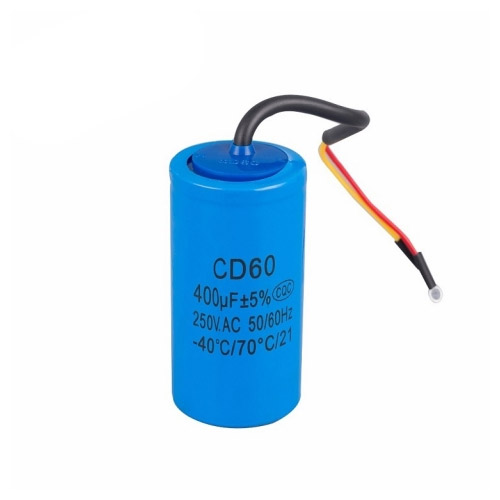
\includegraphics[width=0.3\linewidth]{../figs/C03-BT-02}
\end{center}
\begin{mcq}(4)
	\item $\SI{0.100}{\coulomb}$.
	\item $\SI{0.095}{\coulomb}$.
	\item $\SI{0.105}{\coulomb}$.
	\item $\SI{0.160}{\coulomb}$.
\end{mcq}
\hideall{
\textbf{Đáp án C.}\\
Điện tích tối đa tụ có thể tích được:
$$Q_\text{max}=\left(C+\SI{5}{\percent}C\right)\cdot U_\text{max}=\SI{0.105}{\coulomb}.$$
}

\item Một điện trường đều có cường độ $\SI{4000}{\volt/\meter}$, có phương song song với cạnh huyền BC của tam giác vuông ABC có chiều từ B đến C, biết $\text{AB}=\SI{6}{\centi\meter}$, $\text{AC}=\SI{8}{\centi\meter}$. Hiệu điện thế giữa hai điểm CB
\begin{mcq}(4)
	\item $\SI{400}{\volt}$.
	\item $\SI{240}{\volt}$.
	\item $\SI{-320}{\volt}$.
	\item $\SI{-400}{\volt}$.
\end{mcq}
\hideall{
\textbf{Đáp án D.}\\
\begin{center}
	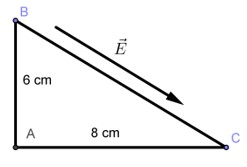
\includegraphics[width=0.3\linewidth]{../figs/C03-BT-01}
\end{center}
$$U_\text{CB}=Ed_\text{CB}=E\cdot \text{CB}\cos\SI{180}{\degree}=\left(\SI{4000}{\volt/\meter}\right)\cdot\sqrt{\left(\SI{0.06}{\meter}\right)^2+\left(\SI{0.08}{\meter}\right)^2}\cdot\cos\SI{180}{\degree}=\SI{-400}{\volt}.$$
}

\item Một hạt bụi khối lượng $\SI{3.6E-15}{\kilogram}$ mang điện tích $\SI{4.8E-18}{\coulomb}$ nằm cân bằng trong khoảng giữa hai tấm kim loại phẳng tích điện trái dấu và đặt song song nằm ngang. Tính cường độ điện trường giữa hai tấm kim loại. Lấy $g=\SI{10}{\meter/\second^2}$.
\begin{mcq}(4)
	\item $\SI{1000}{\volt/\meter}$.
	\item $\SI{75}{\volt/\meter}$.
	\item $\SI{750}{\volt/\meter}$.
	\item $\SI{7500}{\volt/\meter}$.
\end{mcq}
\hideall{
\textbf{Đáp án D.}\\
Hạt bụi nằm cân bằng khi 
$$F_\text{đ}=P$$
$$\Leftrightarrow E=\dfrac{mg}{q}=\SI{7500}{\volt/\meter}.$$
}

\item Hai điện tích $q_1=\SI{4E-8}{\coulomb}$ và $q_2=\SI{-4E-8}{\coulomb}$ đặt tại hai điểm A và B cách nhau một khoảng $\SI{4}{\centi\meter}$ trong không khí. Lực tác dụng lên điện tích $q=\SI{2E-7}{\coulomb}$ đặt tại trung điểm O của AB là
\begin{mcq}(4)
	\item $\SI{36}{\newton}$.
	\item $\SI{0.36}{\newton}$.
	\item $\SI{0}{\newton}$.
	\item $\SI{0.09}{\newton}$.
\end{mcq}
\hideall{
\textbf{Đáp án B.}\\
Lực tác dụng lên điện tích $q$ gồm $\vec{F}_{1q}$ và $\vec{F}_{2q}$ mà $\vec{F}_{1q}\uparrow\uparrow\vec{F}_{2q}$ nên:
$$F=F_{1q}+F_{2q}=\dfrac{k\left|q_1q_2\right|}{OA^2}+\dfrac{k\left|q_1q_2\right|}{OB^2}=\SI{0.36}{\newton}.$$
}

\item Điện tích $q$ di chuyển trong một điện trường đều có cường độ điện trường $\SI{800}{\volt/\meter}$ theo một đoạn thẳng AB. Đoạn AB dài $\SI{12}{\centi\meter}$ và vector độ dời hợp với đường sức điện một góc $\SI{30}{\degree}$. Biết công của lực đinệ trong sự di chuyển của điện tích $q$ là $\SI{-1.33E-4}{\joule}$. Điện tích $q$ có giá trị bằng
\begin{mcq}(4)
	\item $\SI{-1.6E-6}{\coulomb}$.
	\item $\SI{1.6E-6}{\coulomb}$.
	\item $\SI{-1.4E-6}{\coulomb}$.
	\item $\SI{1.4E-6}{\coulomb}$.
\end{mcq}
\hideall{
\textbf{Đáp án A.}\\
Giá trị điện tích $q$:
$$q=\dfrac{A}{Es\cos\SI{30}{\degree}}\approx\SI{-1.6E-6}{\coulomb}.$$
}

\item Một hạt bụi kim loại tích điện âm và có khối lượng $\SI{E-10}{\kilogram}$ lơ lửng trong khoảng giữa hai bản tụ điện phẳng nằm ngang đặt trong không khí, bản tích điện dương ở trên, bản tích điện âm ở dưới. Hiệu điện thế giữa hai bản bằng $\SI{1000}{\volt}$, khoảng cách giữa hai bản là $\SI{4.8}{\milli\meter}$, bỏ qua khối lượng của electron, lấy $g=\SI{10}{\meter/\second^2}$. Số electron dư ở hạt bụi là
\begin{mcq}(4)
	\item $\SI{2.5E4}{\text{electron}}$.
	\item $\SI{3E4}{\text{electron}}$.
	\item $\SI{2E4}{\text{electron}}$.
	\item $\SI{4E4}{\text{electron}}$.
\end{mcq}
\hideall{
\textbf{Đáp án B.}\\
Hạt bụi nằm lơ lửng nên:
$$F_\text{đ}=P$$
$$\dfrac{N\left|e\right|U}{d}
=mg$$
$$\Rightarrow N=\dfrac{mgd}{U\left|e\right|}=\SI{3E4}{\text{electron}}.$$}

\item Hai điện tích điểm $q_1=\SI{-E-6}{\coulomb}$ và $q_2=\SI{E-6}{\coulomb}$ đặt tại hai điểm A và B cách nhau $\SI{40}{\centi\meter}$ trong chân không. Cường độ điện trường tại điểm N cách A đoạn $\SI{20}{\centi\meter}$ và cách B đoạn $\SI{60}{\centi\meter}$ có độ lớn
\begin{mcq}(4)
	\item $\SI{E5}{\volt/\meter}$.
	\item $\SI{0.5E5}{\volt/\meter}$.
	\item $\SI{2E5}{\volt/\meter}$.
	\item $\SI{2.5E5}{\volt/\meter}$.
\end{mcq}
\hideall{
\textbf{Đáp án C.}\\
Cường độ điện trường tổng hợp tại N:
$$\vec{E}_\text{N}=\vec{E}_1+\vec{E}_2$$
Vì $\vec{E}_1\uparrow\downarrow \vec{E}_2$ nên
$$E=\left|E_1-E_2\right|=\left|\dfrac{k\left|q_1\right|}{AN^2}-\dfrac{k\left|q_2\right|}{BN^2}\right|=\SI{2E5}{\volt/\meter}.$$
}

\item Hai điện tích $q_1=q_2=\SI{5E-16}{\coulomb}$ đặt tại hai đỉnh B và C của một tam giác đều ABC cạnh bằng $\SI{8}{\centi\meter}$ trong không khí. Cường độ điện trường tại đỉnh A của tam giác ABC có độ lớn bằng
\begin{mcq}(4)
	\item $\SI{1.2178E-3}{\volt/\meter}$.
	\item $\SI{0.6089E-3}{\volt/\meter}$.
	\item $\SI{0.3515E-3}{\volt/\meter}$.
	\item $\SI{0.7031E-3}{\volt/\meter}.$
\end{mcq}
\hideall{
\textbf{Đáp án A.}\\
Cường độ điện trường tại đỉnh A của tam giác đều ABC:
$$\vec{E}_\text{A}=\vec{E}_1+\vec{E}_2$$
Với độ lớn cường độ điện trường do mỗi điện tích điểm gây ra tại A:
$$E_1=E_2=\dfrac{k\left|q_1\right|}{a^2}=\xsi{\dfrac{9}{12800}}{\volt/\meter}.$$
Vì $\left(\vec{E}_1, \vec{E}_2\right)=\SI{60}{\degree}$ nên 
$$E_\text{A}=2E_1\cos\dfrac{\SI{60}{\degree}}{2}=\SI{1.2178E-3}{\volt/\meter}.$$
}

\item Khi bay từ điểm M đến N trong điện trường đều, động năng của electron tăng thêm một lượng $\SI{250}{\electronvolt}$. Hiệu điện thế giữa hai điểm M và N là
\begin{mcq}(4)
	\item $\SI{-250}{\volt}$.
	\item $\SI{250}{\volt}$.
	\item $\SI{-125}{\volt}$.
	\item $\SI{125}{\volt}$.
\end{mcq}
\hideall{
\textbf{Đáp án A.}\\
Áp dụng định lý động năng cho quá trình chuyển động của electron từ M đến N:
$$\Delta W_\text{đ}=q_eU_\text{MN}$$
$$\Rightarrow U_\text{MN}=\dfrac{W_\text{đ}}{q_e}=\dfrac{\SI{250}{\electronvolt}}{-1e}=\SI{-250}{\volt}.$$

}

\item Hai điện tích $q_1=\SI{2E-6}{\coulomb}$ và $q_2=\SI{-8E-6}{\coulomb}$ lần lượt đặt tại hai điểm A và B với $\text{AB}=\SI{10}{\centi\meter}$. Xác định điểm M trên đường AB mà tại đó $\vec{E}_2=4\vec{E}_1$.
\begin{mcq}(2)
	\item M nằm trong AB với $\text{AM}=\SI{2.5}{\centi\meter}$.
	\item M nằm trong AB với $\text{AM}=\SI{5}{\centi\meter}$.
	\item M nằm ngoài AB với $\text{AM}=\SI{2.5}{\centi\meter}.$
	\item M nằm ngoài AB với $\text{AM}=\SI{5}{\centi\meter}.$
\end{mcq}
\hideall{
\textbf{Đáp án B.}\\
Vì hai điện tích trái dấu nên $\vec{E}_1\uparrow\uparrow\vec{E}_2$ khi M nằm trong đoạn AB.\\
Theo đề bài ta có:
$$E_2=4E_1\Leftrightarrow \dfrac{\left|q_2\right|}{r^2_2}=4\dfrac{\left|q_1\right|}{r^2_1}$$
Thay số ta được $r_1=r_2=\dfrac{\text{AB}}{2}=\SI{5}{\centi\meter}.$
}

\item Một proton bay theo phương của một đường sức điện trường. Lúc ở điểm A nó có tốc độ $\SI{2.5E4}{\meter/\second}$, khi đến điểm B thì tốc độ của nó bằng không. Biết proton có khối lượng $\SI{1.67E-27}{\kilogram}$ và có điện tích $\SI{1.6E-19}{\coulomb}$. Điện thế tại A là $\SI{500}{\volt}$, điện thế tại B là
\begin{mcq}(4)
	\item $\SI{406.7}{\volt}$.
	\item $\SI{500}{\volt}$.
	\item $\SI{503.3}{\volt}$.
	\item $\SI{533}{\volt}$.
\end{mcq}
\hideall{
\textbf{Đáp án C.}\\
Áp dụng định lý động năng cho chuyển động của proton từ A đến B:
$$W_\text{đB}-W_\text{đA}=q\left(V_\text{A}-V_\text{B}\right)$$
$$\Leftrightarrow 0-\dfrac{1}{2}mv^2_0=q\left(V_\text{A}-V_\text{B}\right)$$
$$\Rightarrow V_\text{B}=\SI{503.3}{\volt}.$$
}
\end{enumerate}